\section{Mixture Models \& Secant Varieties}

\begin{frame}{Hidden Variables}
    \begin{itemize}
    \item Suppose $\mc{P} \subset \Delta_{r-1}$ is a model for a random variable $X$ with state space $[r]$.
    \item Moreover, assume that there is a \emph{hidden} or \emph{latent} random variable $Y$ with state space $[s]$, and for each $j \in [s]$, the conditional distribution of $X$ given $Y = j$ is $p^{(j)} \in \mc{P}$. 
    \item The hidden variable $Y$ also has some probability distribution $\pi \in \Delta_{s-1}$.
    \end{itemize}

    So the joint distribution of $Y$ and $X$ is given by the formula
    $$ P(Y = j; X = i) = \pi_{j} \cdot p_{i}^{(j)}. $$

\end{frame}

\begin{frame}{Mixture Models}

    \begin{itemize}
    \item But as $Y$ is hidden, we can only observe the marginal distribution of $X$, that is
    $$ P(X = i) = \sum_{j = 1}^{s} \pi_{j} \cdot p_{i}^{(j)}. $$

    \item In other words, the marginal distribution of $X$ is the convex combination of the $s$ distributions $p^{(1)}, \ldots, p^{(s)}$, with weights given by $\pi$.
    \end{itemize}

    \begin{block}{Definition}
        Let $\mc{P} \subset \Delta_{r-1}$ be a statistical model. The \emph{$s$-th mixture model} is
        $$ \Mixt^{s}(\mc{P}) := \Bigg\{ \sum_{j = 1}^{s} \pi_{j}\cdot p^{(j)} : \pi \in \Delta_{s-1},\ p^{(j)} \in \mc{P}, \text{ for all } j \Bigg\}. $$
    \end{block}

\end{frame}

\begin{frame}{Mixture Models}

    \begin{itemize}
    \item Mixture models provide ways to build complex models out of simpler ones.

    \item Basic assumption is that the underlying population to be modelled can be split into $s$ disjoint sub-populations.

    \item Restricted to each sub-population, the observable $X$ follows a probability distribution from the simple model $\mc{P}$.

    \item After marginalisation though, the structure becomes significantly more complex as it is now a convex combination of these simple distributions.

    \end{itemize}

\end{frame}

\begin{frame}{Phylogenetic Trees}

    \begin{itemize}
        \item Introduce \emph{phylogenetic trees}; describe the descent of species from a common ancestor:        
        \begin{block}{Example Cartoon}

        \begin{center}
        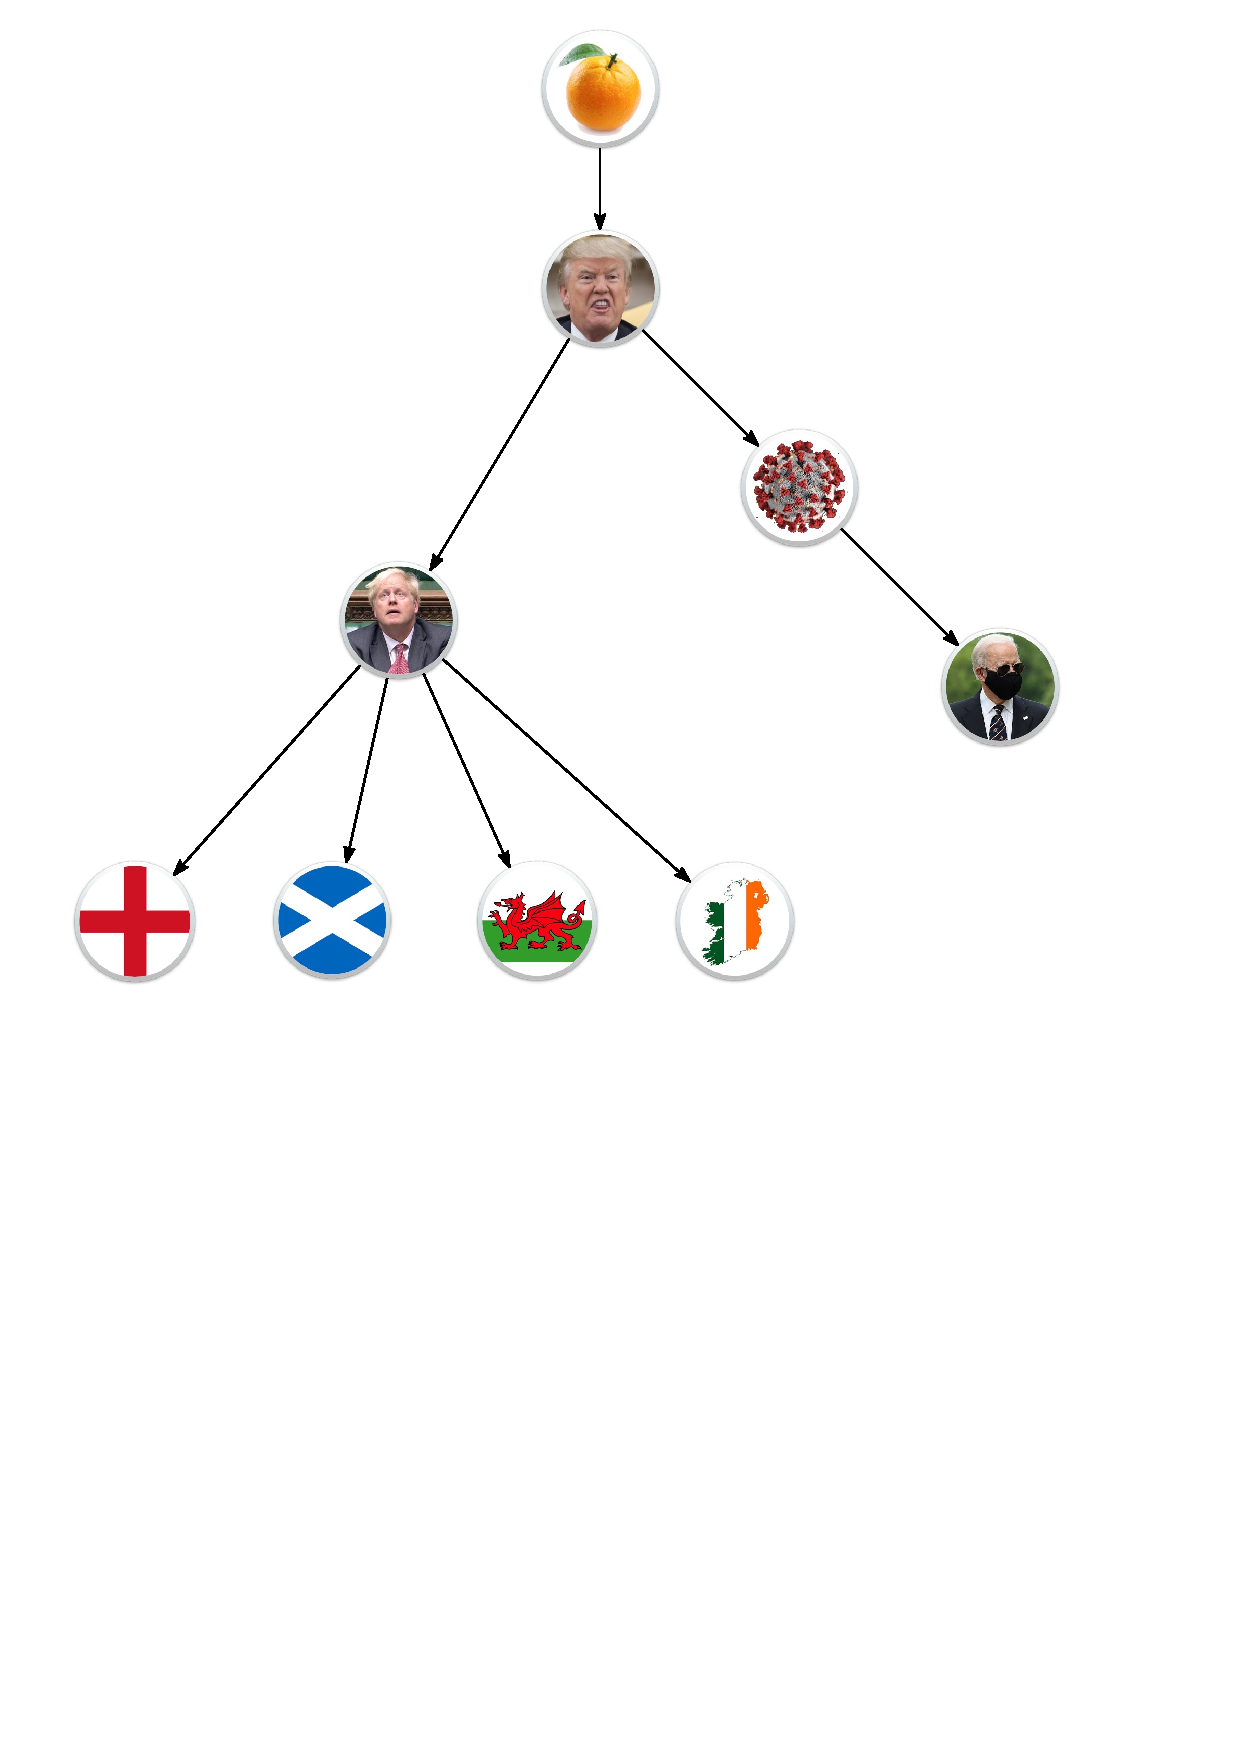
\includegraphics[width=0.5\textwidth, angle=0]{resources/phylogenetic-tree.pdf}
        \end{center}
        \end{block}

    \end{itemize}

\end{frame}

\begin{frame}{Molecular Phylogenetics}

    \begin{itemize}
        \item Sequence of DNA molecules in a genome is represented as a sequence of letters from the four letter alphabet $\Sigma = \{ \texttt{A}, \texttt{C}, \texttt{G}, \texttt{T} \}$.

        \item At a particular site of the genome, any of the four nucleotides $\texttt{X} \in \Sigma$, say, might be observed.

        \item Based on a particular ancestral nucleotide of $\texttt{X}$, might expect evolution to occur in a way that the state of the current nucleotide is independent of one another:

        $$ \texttt{A} \mapsto \texttt{X},\ \texttt{C} \mapsto \texttt{X},\ \texttt{G} \mapsto \texttt{X}, \text{ or } \texttt{T} \mapsto \texttt{X}. $$

        \item So for each ancestral nucleotide, we have an independence model; its distribution is determined by a point of $\Delta_{3} = \Delta_{4-1}$.

    \end{itemize}

\end{frame}

\begin{frame}{Example}
    \begin{itemize}
        \item  $X$ is a hidden variable though; could have been any one of $\texttt{A}, \texttt{C}, \texttt{G}$, or $\texttt{T}$.

        \item For \emph{exactly one choice} of $X$, we had the distribution $\Delta_{3}$; need to consider \emph{all choices} of ancestral nucleotide.

        \item Hence we get the mixture model: $\Mixt^{4}(\Delta_{3}) =$

        $$\Bigg\{ \sum_{i = 1}^{4} \Prob(X = i)\cdot \lambda_{i}  :\ i \in \Sigma,\ \lambda_{i} \in [0,1],\ \lambda_{1} + \ldots + \lambda_{4} = 1 \Bigg\}. $$

        \item \textbf{Q?}: What is the analogue for mixture models in algebraic statistics?
    \end{itemize}
\end{frame}

\begin{frame}{Secant Varieties}
    \begin{itemize}
        \item \textbf{A!}: Secant\footnote{from \emph{secare}, ``to cut'' in Latin; \emph{c.f. tangō}, ``to touch''.} varieties!
    \end{itemize}

    \begin{block}{Definitions}
        \begin{itemize}
        \item Consider two varieties $V, W \subseteq \RR^{k}$. The \emph{join} of $V$ and $W$ is the variety
        $$ \mc{J}(V,W) := \{ \lambda v + (1-\lambda)w : v \in v, w \in W, \lambda \in [0,1] \}. $$

        \item If $V = W$, then this is the \emph{secant variety} of $V$, denoted $\Sec^{2}(V) = \mc{J}(V,V)$. The \emph{$s$-th higher secant variety} is:
        $$ \Sec^{1}(V) := V, \qquad \Sec^{s}(V) := \mc{J}(\Sec^{s-1}(V), V ). $$
        \end{itemize}
    \end{block}

\end{frame}

\begin{frame}{Secant Varieties}
   
    \begin{center}
        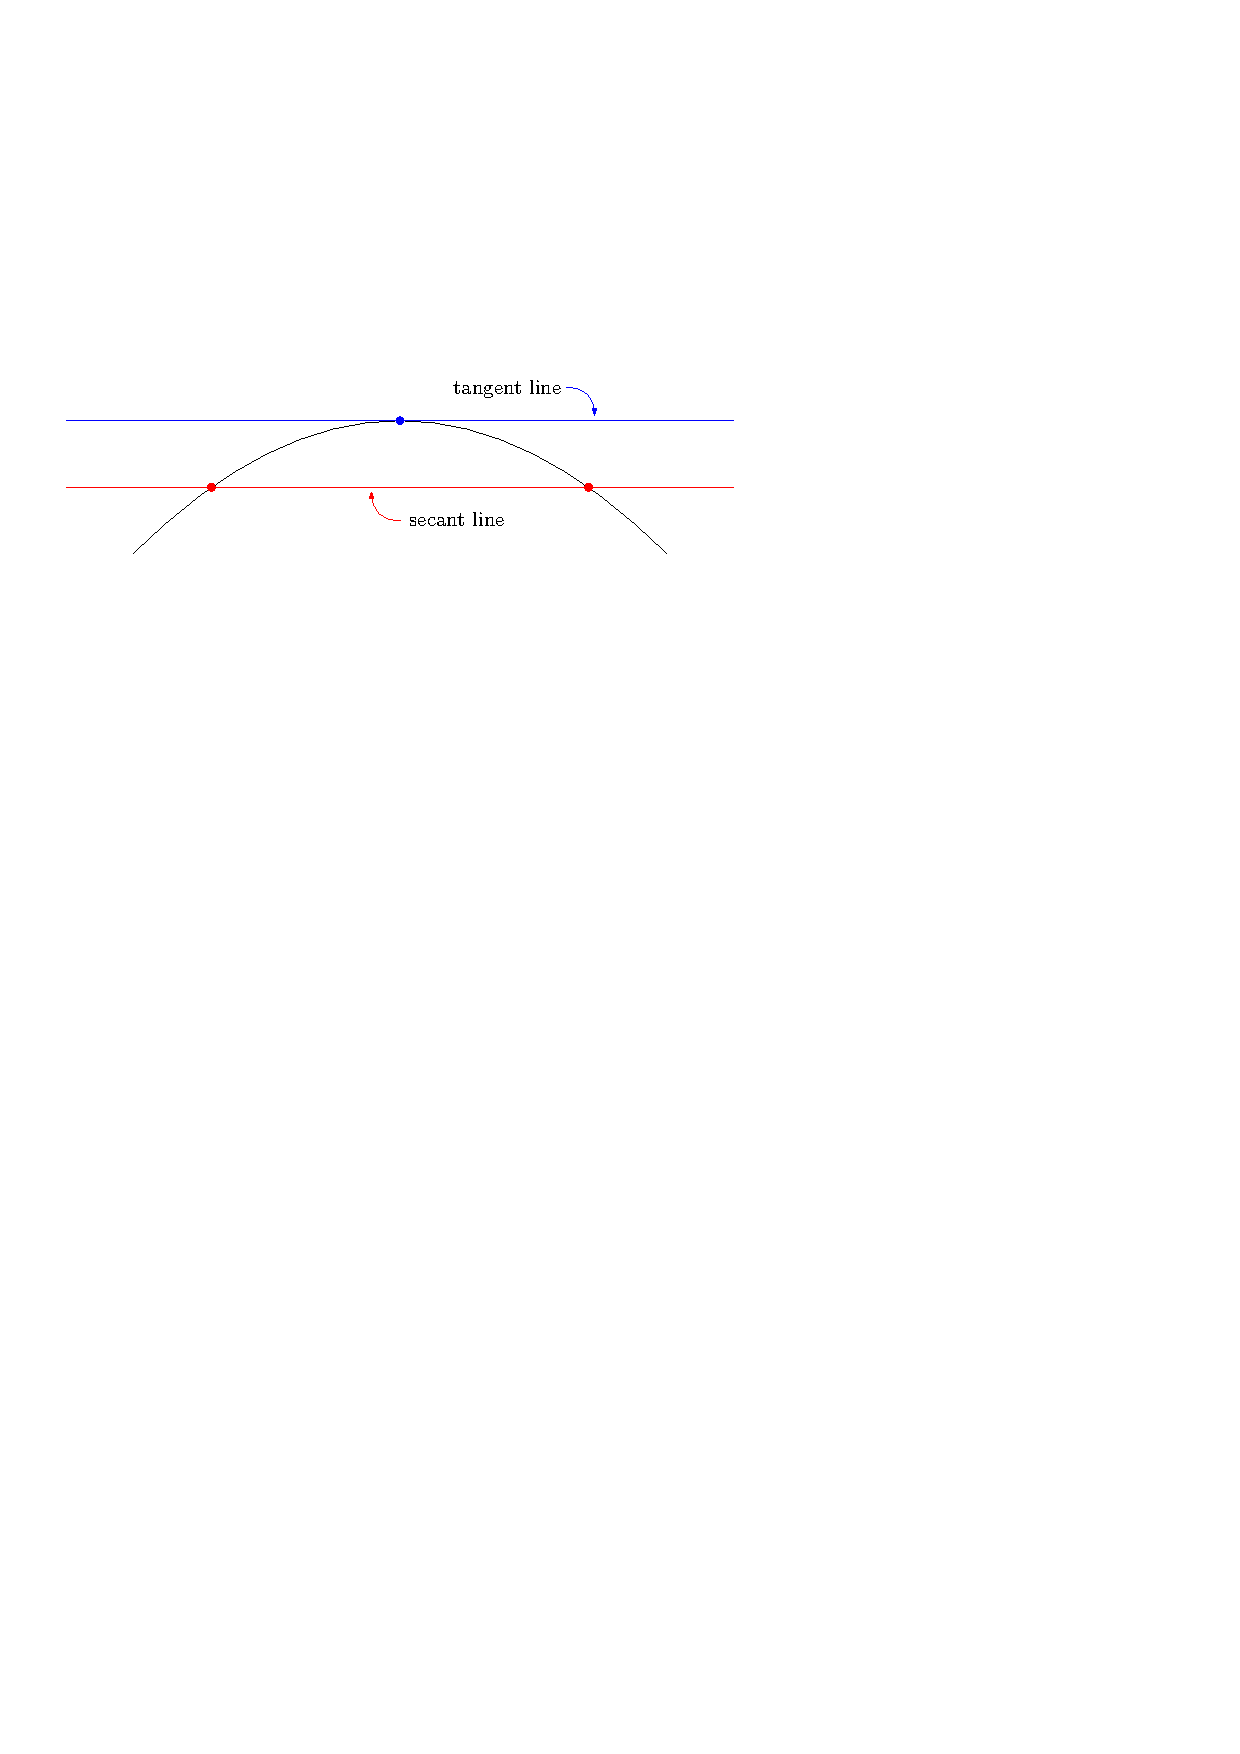
\includegraphics[height=0.25\textwidth, angle=0]{resources/secant-line.pdf}
    \end{center}

    \begin{center}
        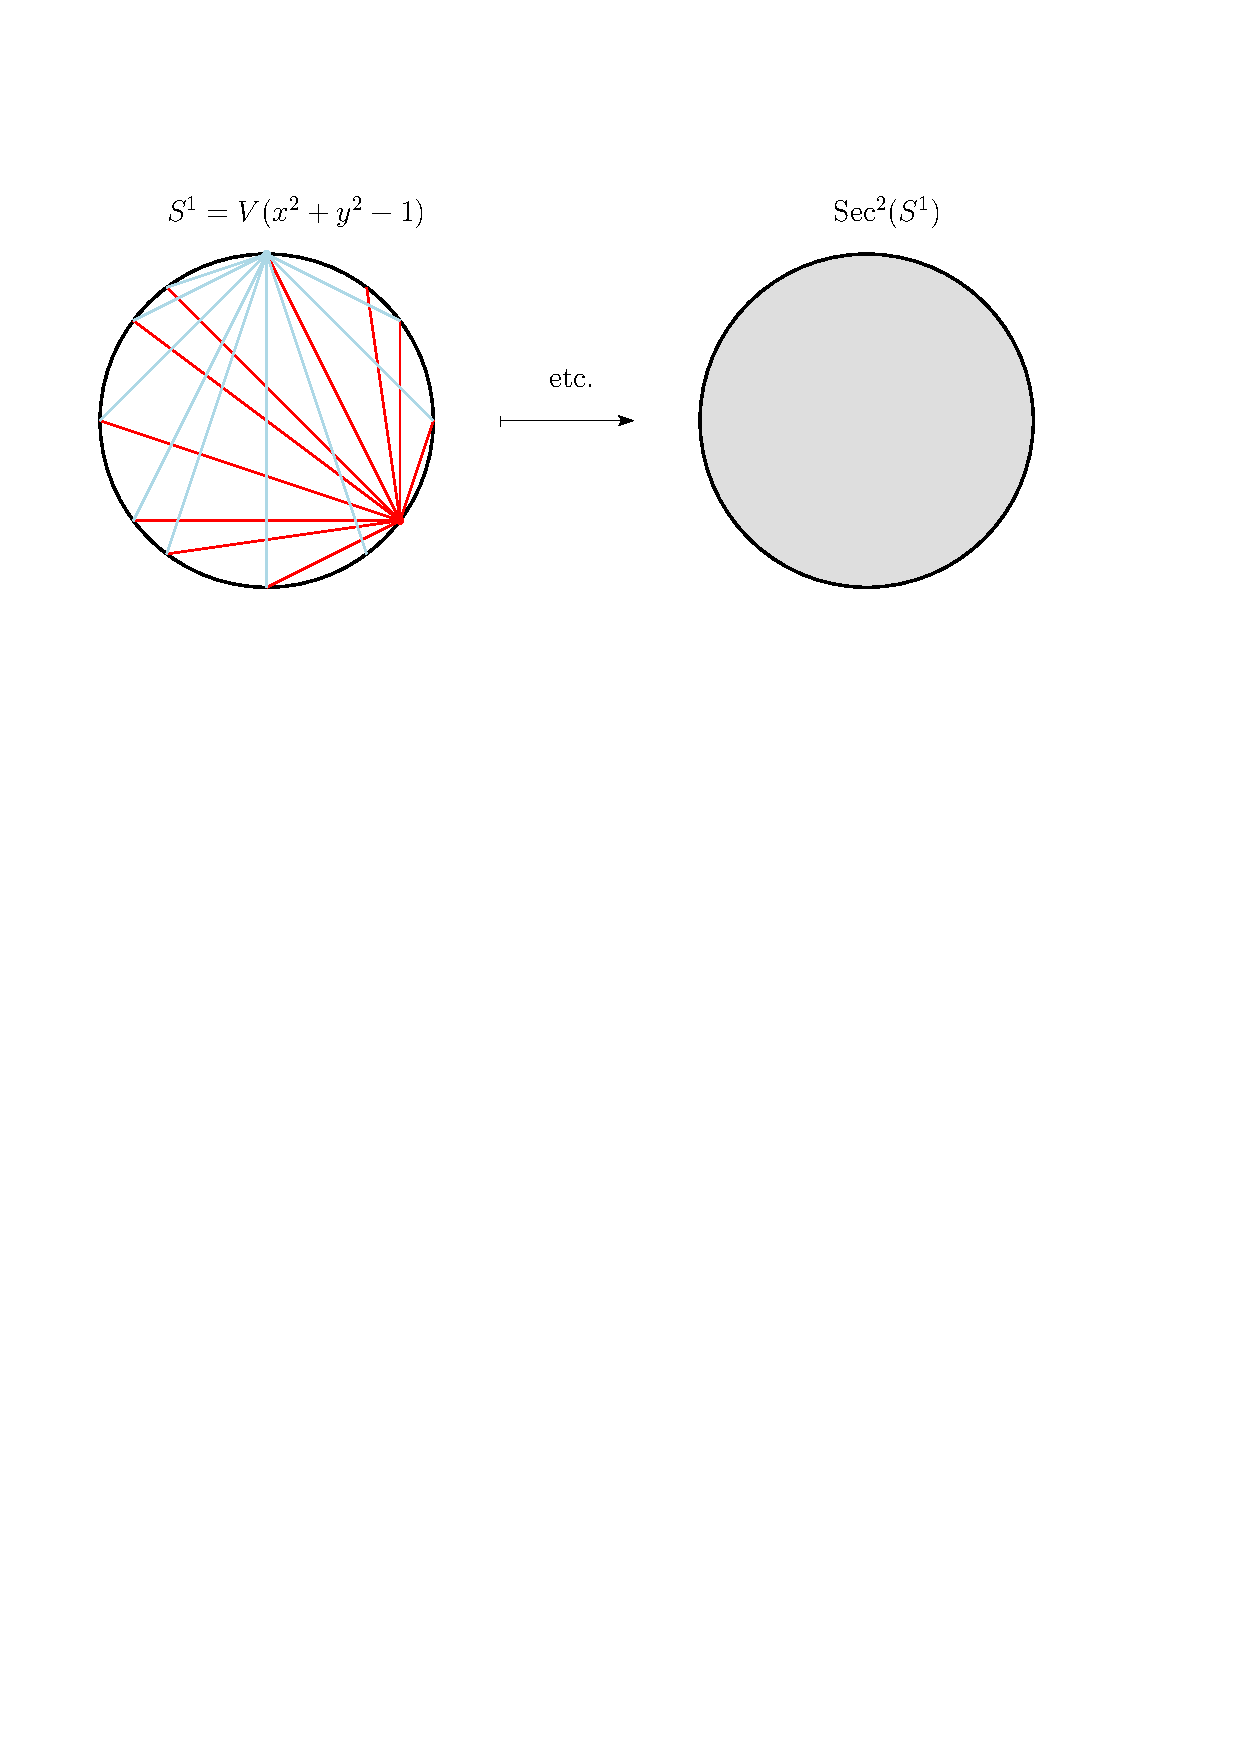
\includegraphics[height=0.35\textwidth, angle=0]{resources/secant-circle.pdf}
    \end{center}

\end{frame}

\begin{frame}{More Complicated Phylogenetic Trees}

    \begin{itemize}
        \item Last example only had one extant species; $X \overset{?}{\longmapsto} \texttt{A}, \texttt{C}, \texttt{G}, \texttt{T}$.

        \item What if we had three extant species, coming from one ancestor?

    \begin{center}
        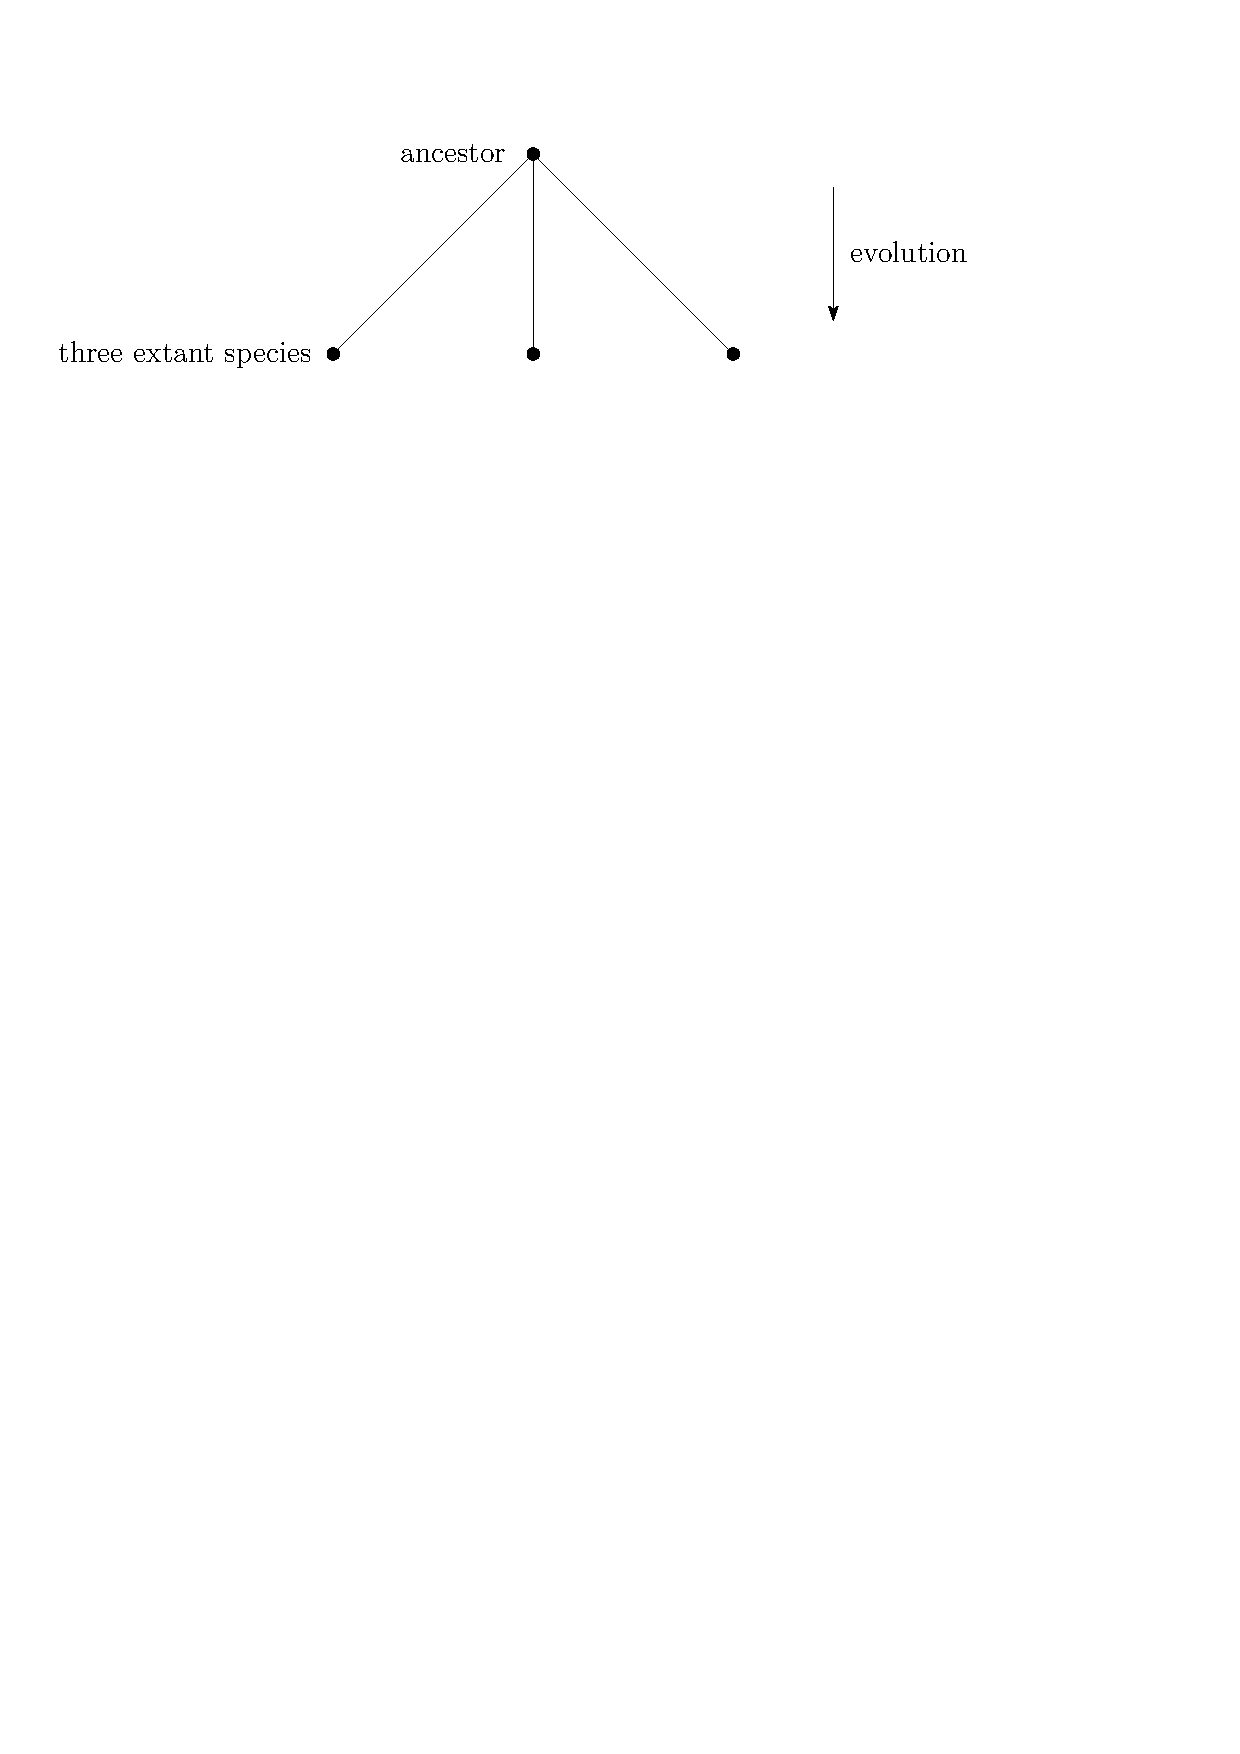
\includegraphics[width=0.6\textwidth, angle=0]{resources/three-extant.pdf}
    \end{center}

    \item Now we have to consider: $\Sec^{4}(\PP^{3} \times \PP^{3} \times \PP^{3})$; or equivalently $\Mixt^{4}(\Delta_{3} \times \Delta_{3} \times \Delta_{3})$.

    \item Finding the minimal set of polynomials defining $\Sec^{4}(\PP^{3} \times \PP^{3} \times \PP^{3})$ once gave rise to a very important application of algebraic statistics...

    \end{itemize}

\end{frame}

\begin{frame}{The \emph{Salmon Problem}}

\begin{block}{Statement}
    \emph{Determine the ideal\footnote{read this as ``set of defining polynomials''.} defining $\Sec^{4}(\PP^{3} \times \PP^{3} \times \PP^{3})$.}
\end{block}

\begin{block}{Prize}
    Personally caught, and smoked just for you, copper river salmon from Alaska.
\end{block}

\begin{block}{Current Status}
    Solved.
\end{block}

\begin{itemize}
    \item At an IMA workshop in 2007, Elizabeth Allman offered this prize to whomever solved the above problem.
    \item It was solved in 2010 by Shmuel Friedland.
\end{itemize}

\end{frame}

\begin{frame}{}

\begin{itemize}
    \item 
\end{itemize}

\end{frame}